\chapter{相关背景}
\label{chap:background}
本章将对相关背景进行介绍。~\ref{sec:android-perm}节和~\ref{sec:background-appaudit}节分别介绍了Android权限机制以及单应用审查工具;~\ref{sec:sim-detect}节中介绍了相似度检测;~\ref{sec:obfuscation}节中介绍了Android混淆相关概念以及技术;~\ref{sec:background-conclusion}节对本章进行了小结。

\section{Android权限机制}
\label{sec:android-perm}

Android的权限控制分为几个层面,系统层面和应用层面。
在系统层面,Android是运行在Linux内核之上的,Linux内核已经经过多年广泛的使用,而且很多对安全敏感的环境都在使用Linux。
Linux一直活跃在研究领域,经过数十年的发展与修正,已经成为了一个稳定且安全的操作系统内核。
作为移动计算的基础,Linux内核为Android操作系统提供了很多关键的安全特性:

\begin{enumerate}
  \item 基于用户的权限模型
  \item 进程隔离
  \item 可拓展的安全进程内通信
\end{enumerate}

Linux作为一个多用户操作系统,一个基本的安全规则就是隔离不同用户的资源。
在Linux中,一个用户不能读另一个用户的文件、一个用户不会耗尽另外一个用户的资源,如内存、CPU以及硬件设备等。

Android平台利用了Linux的基于用户粒度的保护这一特点,实现了识别并且隔离不同应用的资源。
在安装应用时,Android操作系统会给应用分配一个独特的系统标识,即Linux的UserID和GroupID。
在运行应用时,Android会让这个应用跑在所述用户单独的进程下。
这跟很多其他的操作系统,包括Linux的传统用法不同,一般的做法都是多个应用会运行在同一个用户下面。

这种做法建立了一个内核级别的应用沙盒,使得不同应用之间的资源通过不同的UserID和GroupID实现了隔离。
由于这个沙盒是建立于内核级别的,无论是应用代码、Dalvik虚拟机还是支持库都无法越权访问属于其他进程(应用)的数据。

其中root为最高权限的用户,可以访问任何权限,在Android中只有内核以及小部分核心系统应用是以root权限运行的。在一般情况下,root权限是不会开放给用户的,这是为了保护用户的root权限不被恶意应用所利用。

在应用层面,默认情况下,一个应用只能访问有限的系统资源,这是为了保护用户的数据以及硬件不被误用或者恶意使用。
Android通过多种方式来实现对应用的限制,有些功能直接不提供API来操作,例如没有Android API直接操作SIM卡。
同时,一些可能会使用重要资源的敏感API只会提供给被信任的应用使用,这种机制就是我们经常说到的权限。

在Android系统中,受到保护的API主要有以下几类:

\begin{enumerate}
	\item 摄像头功能
	\item 位置信息
	\item 蓝牙功能
	\item 通话功能
	\item 短信、彩信功能
	\item 网络连接
\end{enumerate}


这些资源只允许操作系统访问。
如果一个应用想要使用这些资源,必须在Manifest中声明使用对应的Capabilities。
如图~\ref{fig:android-perm},需要监控传入的短信的应用要在Manifest指定声明android.permission.RECEIVE\_SMS。
当安装应用时,系统会弹窗描述该App需要获取的权限,用户只有允许才能安装使用。
如果用户继续安装,系统则会认定用户已经授予了应用使用要求的权限。
用户要么全部接受,要么拒绝安装,用户无法拒绝某一项权限。

\begin{figure}
	\centering
	\begin{lstlisting}[language={xml}]
	<manifest xmlns:android="http://schemas.android.com/apk/res/android"
		package="com.android.app.myapp" >
		<uses-permission android:name="android.permission.RECEIVE_SMS" />
		...
	<manifest/>
	\end{lstlisting}
	\bicaption[fig:android-perm]{AndroidManifest.xml中声明监控接收短信的权限}{AndroidManifest.xml中声明监控接收短信的权限}{Fig}{Using RECEIVE\_SMS Permission in AndroidManifest.xml}
\end{figure}

在Android 6.0版本后加入了运行时授予权限的功能\footnote{Android Permission: \url{https://developer.android.com/training/permissions/requesting.html}},使得用户是在应用运行时向Android授予权限,而不是在应用安装时授予。
此方法可以简化应用安装过程,因为用户在安装或更新应用时不需要授予权限。
同时用户可以准确知道应用会在什么操作时需要什么权限,可以细化权限的使用。

\section{单应用审核工具AppAudit}
\label{sec:background-appaudit}

虽然Android的权限机制能够在应用的使用中有效的展示其使用了哪些敏感资源,但是无法追踪应用是如何使用这些敏感资源的。
以“滴滴出行”应用程序为例,在安装时,系统会弹出提示框描述该应用需要获取的权限.
用户无法授权其中一个或几个权限,只能全盘接受或者不予安装。
如图\ref{fig:didi}所示,用户在安装时被提醒“滴滴出行”应用在运行时需要读取内部存储、拨打电话、读取讯息获得精确位置等权限。
而从权限列表中,用户却无法得知应用是如何使用这些权限,比如应用需要获得短信的原因、应用是否会将用户短信通过网络或者其他方式泄露出去。
这些都给了恶意软件可乘之机,导致用户处于隐私数据泄露的威胁之中。

\begin{figure}
	\centering
	\subfigure[]{
		\label{fig:didi:a}
		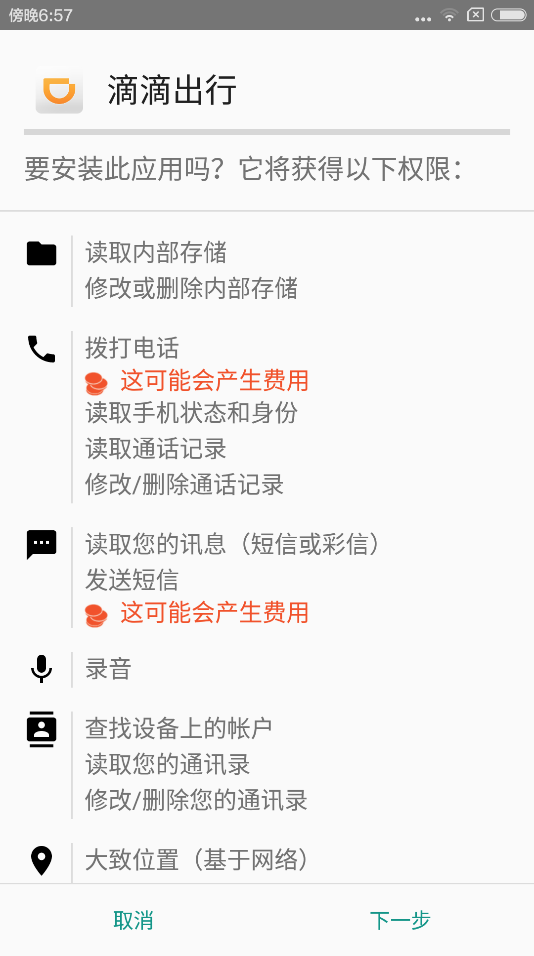
\includegraphics[width=0.4\textwidth]{figure/didi-a.png}
	}
	\hspace{1in}
	\subfigure[]{
		\label{fig:didi:b}
		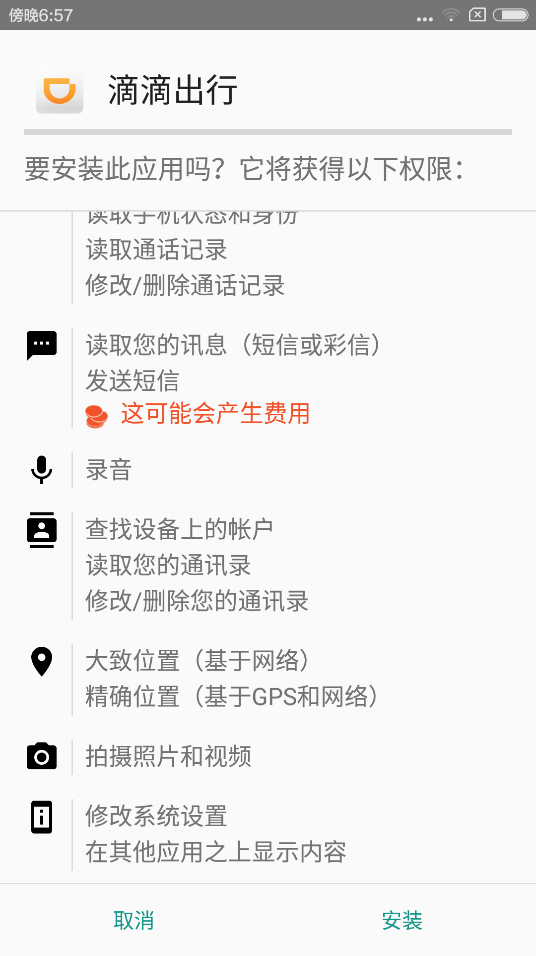
\includegraphics[width=0.4\textwidth]{figure/didi-b.png}
	}
	\bicaption[fig:didi]{“滴滴出行”安装时显示的权限列表}{“滴滴出行”安装时显示的权限列表}{Fig}{Requested Permission List When Installing "DiDiChuXing"}
\end{figure}

为了解决隐私泄露问题,很多应用市场都使用了很多方法来对上传至市场的应用进行审核,从而识别并剔除存在隐私泄露问题的应用程序。
例如,Android在4.2版本中引入了AppVerfiy的服务。
使用了该服务的手机会在安装新应用时,将应用的相关信息,比如应用包名称、SHA-1值等信息提交给AppVerfiy服务器。
服务器会根据这些信息去识别应用是否为已知的恶意软件,最终报告给用户该应用是否会泄露隐私数据。
但由于获得信息有限并且恶意软件发布者可以通过简单的更改包名来绕过检查,所以AppVerfiy的准确率有限~\supercite{appverify}。

在近几年来,很多研究都将程序分析的方法~\supercite{appintent,flowdroid,pios,zhang2013vetting,jiang2013detecting}引入到了移动应用的隐私泄露问题检测中。
这些研究一般分为两种,静态分析和动态分析。
静态分析是指通过对代码进行数据流等方法进行分析,最终找出敏感信息泄露的代码路径。
而动态分析是指在代码运行过程中,通过注入等方法监控程序运行状态,从而在敏感信息泄露发生时将其阻挡。
AppAudit结合了动态和静态的分析方法,分别避免了静态分析内存占用大,分析时间长和动态分析开销大,效率低,覆盖率低的缺点。
AppAudit利用的模糊执行的方法极大程度的减少了分析时的内存占用以及分析时间。
使得AppAudit可以在200多MB、几秒内完成对一个应用的分析。
从图~\ref{fig:appaudit:time}和图~\ref{fig:appaudit:accuracy}中可以看出,AppAudit的分析时间远少于其他同类型工具,同时还能保证比较高的准确率。

\begin{figure}
	\centering
	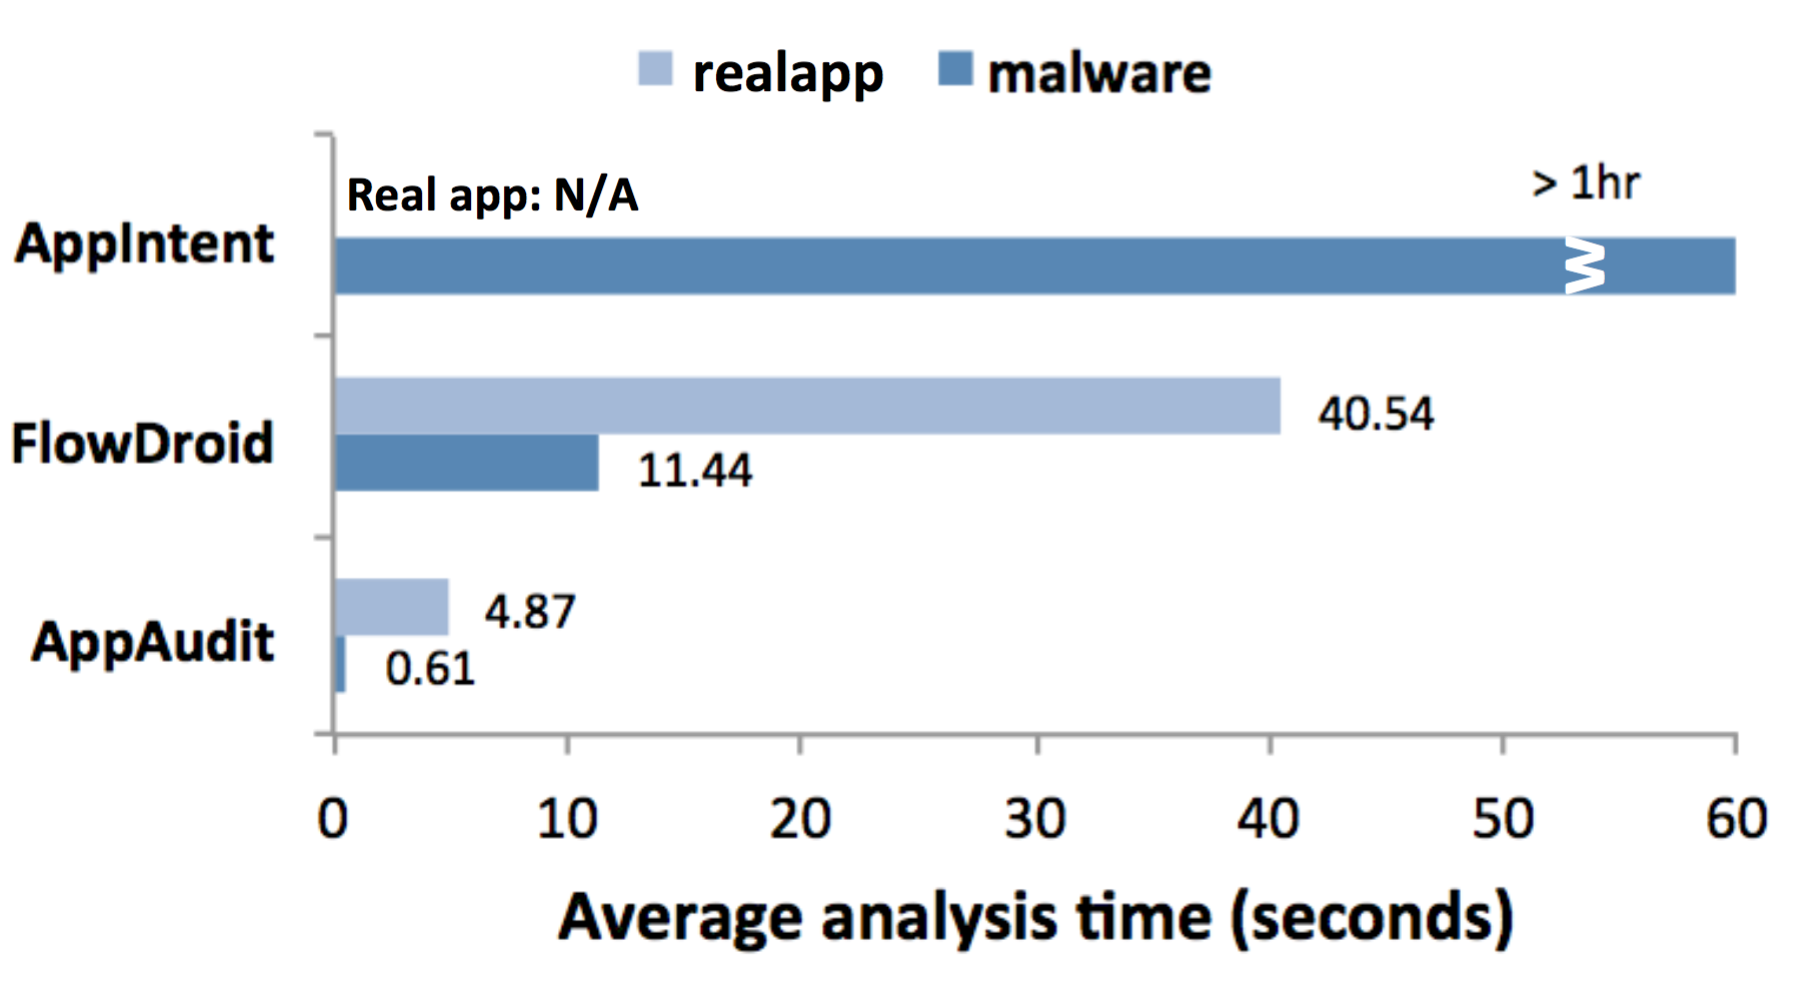
\includegraphics[width=0.7\textwidth]{figure/appaudit-time.png}
	\bicaption[fig:appaudit:time]{AppAudit与其他工具分析时间对比}{AppAudit与其他工具分析时间对比~\supercite{appaudit}}{Fig}{Analysis Time Comparison between AppAudit and Other Tools}
\end{figure}

\begin{figure}
	\centering
	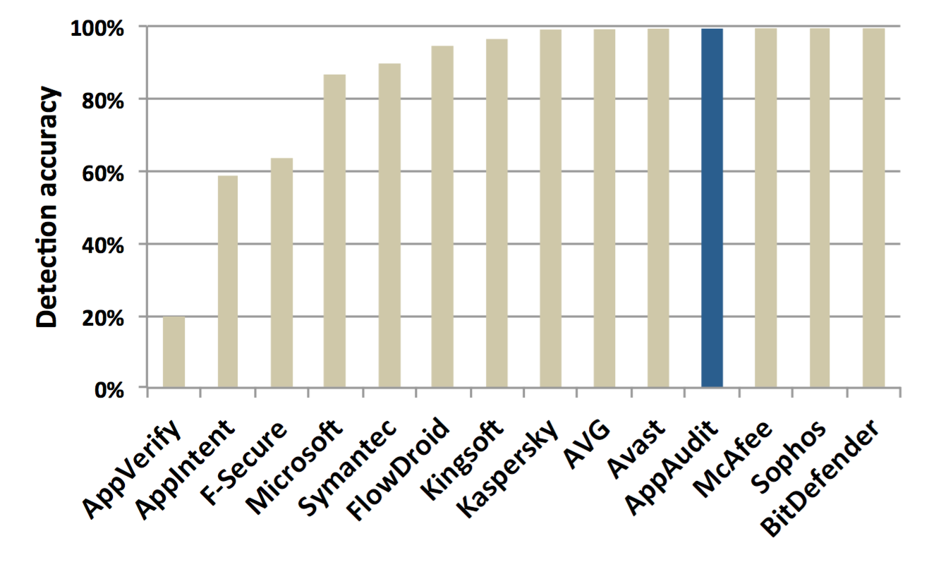
\includegraphics[width=0.7\textwidth]{figure/appaudit-accuracy.png}
	\bicaption[fig:appaudit:accuracy]{AppAudit与其他工具的准确性对比}{AppAudit与其他工具的准确性对比~\supercite{appaudit}}{Fig}{Detection Accuracy Comparison between AppAudit and Other Tools}
\end{figure}

\section{相似度检测}
\label{sec:sim-detect}

第三方库是现代程序开发过程中无法缺少的一部分。
开发者通常会将经常复用的代码以库的形式打包,来加速软件开发,而发布给他人使用的库则成为第三方库。
在Android应用开发中,常见的第三方库种类有工具类库,比如gson,okhttp等、广告类库,如Tapjoy,Admob,还有数据统计类库Google Analytics,TalkingData等等。
由于第三方库的质量参差不齐,开发者使用的第三方库可能会给应用带来相应的隐私问题。
最近研究表明~\supercite{enck:androidsec,grace2012unsafe},很多有名的第三方库会泄露用户的隐私信息。
此外由于第三方库广泛的运用于应用开发中,第三方库占应用代码大多数比例是很常见的情况。
这对Android应用程序分析带来了额外的开销于噪音,所以很多程序分析需要先排除掉第三方库来是的分析过程更高效准确。
例如在检测克隆应用时,需要排除掉第三方库对结果造成的影响。

另外,当在应用审查中,如果不能有效的检测出应用包含的第三方库,那么在应用出现隐私泄露或者安全漏洞时,无法定位。
如今有很多安全相关的分析工具能对应用很多方面进行分析,包括隐私泄露~\supercite{androidleaks, flowdroid, amandroid, droidsafe,rdroid}、权限使用检查~\supercite{remystified}、动态代码加载~\supercite{execute}、SSL/TLS安全相关问题~\supercite{topin, eve}等等。
如果不能在将第三方库和开发者本身的代码区分开,我们就很难确定,存在的问题到底是开发者有意为之还是只是因为引入了一个有问题的第三方库。

第三方库的检测可以通过检测应用与第三方库之间的组件相似程度来实现。
而这种相似度检测的方法也可以应用与克隆应用检测中,如果检测到两个应用相似度很高,并且两个应用的开发者密钥不同的话,这对应用就为一对潜在的克隆应用。

在检测过程中,最大的挑战来自于混淆。
代码混淆是现代软件开发中一个常用的技术,是指将程序代码做一种变形,在不影响程序功能的情况下,使得反编译后的代码难于阅读和理解。
代码混淆能够有效地增加逆向工程的难度,使得软件破解与注入的成本大大增加。
另外在移动应用开发中,代码混淆还能通过将代码中的各种变量名重命名成短名称,来有效的减少应用的代码体积,从而对应用包进行“瘦身”。
而混淆过程中,应用的代码会发生改变,会使得针对应用代码的程序分析变得困难。

\section{Android混淆技术}
\label{sec:obfuscation}

Android应用是使用Java语言进行开发。
使用Java开发的一个主要好处就是可移植性,编译好的程序可以跑在大多数平台上。
Android应用在构建过程中会首先被编译成Java字节码,最终通过Dalvik编译器编译成平台无关的Dalvik字节码,最终运行在Dalvik虚拟机上。
为了节省空间,Java会将所有类型名、变量名和方法名全部存储在常量库中。
而Dalvik在编译过程会把所有Java字节码文件合并压缩成一个Dalvik字节码文件,多个常量库也会合并成一个,从而使得多个类共用的资源只需要存成一份,节约空间。
这些常量库和指令为虚拟机还原Java语义。

由于字节码的语义丰富,已经有很多成熟的反编译软件,例如jd, jadx, dex2jar等等。
经过反编译软件处理后的程序代码已经可以基本上和源代码相同。
这些反编译软件极大程度上威胁了软件作者的权益。
不法分子可以通过反编译来破解软件、加入恶意代码后将软件重新发布等等。

混淆工具是防御反编译威胁的主要方式之一。
混淆会在不改变代码功能的同时,改变代码的形式,使得代码变得更加模糊。
混淆的目标是使得反编译后的程序难以被理解,从而使破解者需要花费更多的时间与精力在混淆代码上。
在混淆中,被混淆的部分成为混淆范围。
在开发中,很多库会指定在混淆中需要将其排除在混淆范围之外,以防未知的错误。
而开发者也有时需要指定某个类或者某个包不需要被混淆,来保证程序的正常运行。

在混淆中最常用的几种方式为标识符重命名、代码缩减、包结构重组织。
值得注意的是,很多混淆器也可以对字节码进行优化。
类的成员方法和成员变量可能会在优化的过程中发生变化,所以字节码的优化也可以被视为一种混淆。
接下来会分别介绍以上所说的这几种常用的混淆技术。

\subsection{标识符重命名}
标识符重命名是最基本的一种方式,在Java语言规范中规定到,一个Java程序的标识符包括:
\begin{itemize}
	\item 包
	\item 类型(类或者接口)
	\item 值域
	\item 方法
	\item 参数(方法参数、构造函数参数或者exception handler)
	\item 本地变量
\end{itemize}

但是并不是所有的标识符在编译之后都会保留在字节码中,参数和本地变量可能会在编译的过程中转化成本地变量数组的内存地址。
如果是在调试模式下编译字节码的话,参数和本地变量的名字就会保留在字节码中的LocalVariableTable中。
虽然去除掉LocalVariableTable也会使得反编译变得更困难,但是一些先进的反编译器已经可以自动推测参数以及本地变量名,既然无法阻止自动推测,那么在LocalVariableTable中的名字就不需要被混淆选中进行重命名。
所以只有前五种标识符会被混淆进行重命名。

另外,也并不是所有标识符都能被重命名的。
Dalvik虚拟机在运行时是动态加载并链接引用类型的。
之前提到类名、方法名都是位于字节码的常量池中。
因此,只有在混淆范围内使用的标识符能够被重命名。如
果标识符在混淆范围外的代码中被使用,那么此标识符就不能够被重命名,例如一些类库和标准库。
除此之外还有以下四类标识符是不能被混淆的:
\begin{enumerate}
	\item 实现了某个在混淆范围外的父类或者接口的纯虚方法的方法
	\item 重写了某个在混淆范围外的父类的方法
	\item 开发者指定的不被混淆的标识符
	\item 充当回调函数的方法
\end{enumerate}
当一个应用被反编译后,破解者不仅仅是从标识符的名字来理解标识符所代表的意义,标识符的上下文同时也能反映出一定的信息。
在重命名标识符时,混淆器会充分利用重载来复用标识符的名字,并且会根据字典序来顺序的为标识符重命名,使其成为无意义的名字。
经过重命名后,破解者只能通过代码的上下文来猜测标识符所代表的意义,从而使得破解者理解代码的过程更加困难。
在混淆时一个额外的好处就是字节码的体积会因为更短的标识符名字和标识符名字的复用而减少。

在Java应用中,一个应用时由一个或多个包组成的。
包的作用是组织类,一个包中包含零个或多个类、接口或者子包。
另外包也决定了类的命名空间,包采用树形的存储方式,在一个包中的类、接口和子包的名字不能相同,但是在不同包中的类、接口或者子包,名字可以相同。
通过字典序来顺序生成标识符名字为混淆的一个功能,而顺序生成的步骤会在每个包中重新开始。

根据以上规则,混淆器会对混淆范围内所有可以被混淆的标识符进行重命名,并且在顺序生成标识符的过程中,会在不同包内尽可能的重用标识符的名称。
另外混淆器会充分利用重载来重用标识符,来同时达到混淆代码以及节省空间的作用。

\subsection{代码缩减}

在应用开发中,实际运行的代码可能只是总代码的很小一部分。
特别是在开发者引入了一些第三方库时,这个情况非常常见。
因为第三方库通常会提供一组或多组程序功能,而在开发中可能只会用到其中的小部分。
所以第三方库的代码就会存在大量的冗余,导致代码体积不必要的增大。
在很多混淆器中,也会提供代码缩减的功能。
代码缩减是指把代码中未被调用的方法,和未被引用的类移除,从而减少代码体积,节省空间。

\subsection{包结构重组织}
通常,提供一组相同功能的类和接口会被组织到一个包中,以便于类的查找和使用。
开发者通过包的结构来组织程序的构成。与此同时包结构也会给破解者提供信息来分析字节码。
破解者在理解了包中的一些类后,理解同一个包中其他类就变得更加简单了。

包的另外一个作用是控制包内成员的可访问性。
一个类T中的成员如果被声明为protected,那么只有和T在同一包中的类型和T的子类型能访问此成员。
如果一个类T中的成员没有声明访问类型(默认情况下),那么只有在和T在同一包中的类可以访问其成员。

包结构重组织会打乱原本的包结构,把一些包或者类重新组织到新的包或已有的包中。这样破解者就没法利用包结构这个信息来理解程序从而进行破解。
但重新组织包结构可能会带来一定的副作用,比如破坏原来的包访问权限,因为对包进行了重新组织,一些类或者类中成员的可访问性拓宽。
庆幸的是,扩充字节码的访问范围并不会影响字节码中的指令,从而不会对程序的行为造成影响。

\subsection{字节码优化}

\begin{enumerate}
	\item 死代码移除
		在代码缩减过程中,已经会移除掉没有被调用的方法以及没有被使用的类。
		然而在代码缩减处理后保留下来的方法和类中还会存在着没有被执行的代码。
		优化器可以利用分析变量的活性来判断代码是否真的需要被执行。
		如果一个函数调用没有使得调用的类状态发生改变,我们称这个函数调用是没有“副作用”的。
		如果一个没有“副作用”的函数调用返回值没有被使用,此时这个函数调用也会被移除。
	\item 接口和类合并
		在很多混淆器中,会通过减少类和接口的数量来减少类的数量从而减少代码体积。
		把多个接口合并成一个可能会使得只实现单个接口的类变得不完全。
		这在Java语言层面是不合法的。
		在Java语言规范中提到,除了abstract类,其余类的所有继承的接口的abstract方法必须被实现,无论是在此类或是在此类的父类中。
		但是根据Java语言规范中的二进制代码兼容性章节所述,向一个接口中添加一个abstract方法不会破坏已有二进制代码的兼容性,所以接口合并这种优化方法是可以应用在字节码层的。
	\item 其他
		混淆器可能还会用到一些其他的代码优化技术,比如移除未使用的参数,改变类和方法的访问权限等等。
\end{enumerate}

\subsection{本章小结}
\label{sec:background-conclusion}

在本章中主要介绍了在本论文中用到的相关技术与背景,其中包括四大部分,第一部分介绍了Android的权限机制;第二部分介绍了本论文使用的单应用审查工具AppAudit;之后第三部分介绍了相似度检测相关背景;最后介绍了在相似度检测中遇到的挑战,混淆的相关知识。